

\documentclass[final]{beamer}
\mode<presentation>

% STEP 1:
% Please use 'XeLaTex' or 'LuaLaTex' compiler. To select one of them, click on the 'Menu' button in the left corner and select one of the above-mentioned-compiler.

\usepackage[english]{babel}
\usefonttheme{serif}

% This poster is designed for a three-column recommended style. For two or four columns, you will have to change '.sty' files accordingly.
\usepackage[orientation=portrait,size=a0,scale=1.2]{beamerposter}
\usetheme[COM, threecolumn]{HYposter}

%Remember to change the name of .bib file if you have uploaded with a different name

\addbibresource{bibliography.bib}

% STEP 2: Set up the title and author info
\titlestart{UDINDER}% First two words are yellow
%To keep title all grey, just comment out the above \titlestart command.
\titleend{ APP FOR UNIVERSITY DATES} % second line of title
\titlesize{\veryHuge} % Use this to change title size if necessary. possible sizes are 'small', 'large', 'Large', 'LARGE', 'huge','Huge', 'veryHuge', VeryHuge', 'VERYHuge'. 

\author{
  \small Nicolas Avendaño Barajas \\
  \footnotesize{20231020113}, \\Advanced-programming, \\Distrital university\\
  \and
  \small Juan Sebastian Vega Diaz \\
  \footnotesize{20231020087}, \\Advanced-programming, \\Distrital university}

% Read the docs if you need to add the logo(s) of institutes involved in this work. 
\leftcorner{{
\includegraphics[height=10cm]{flames/logo.png}}}

%These are the recommended font styles. If you want to change to something else, you might need to work with the '.sty' files.

\setmainfont{Georgia}
\setsansfont{Arial}

\begin{document}

\begin{poster}

% STEP 3: Add the contents of your poster between \begin{poster} and \end{poster}

% Use the '\newcolumn' command to create a column at a specific place. If the text of a paragraph does not fit into a column, you can use this command to start a new column. 

\newcolumn
\section{Introduccion}
\justifying
UDInder aims to address the modern challenges of connecting people in the digital age. With the proliferation of dating apps, there's a need for a platform that fosters meaningful connections beyond superficial interactions. This section briefly discusses the evolution of dating apps and highlights the existing gaps in user experience and privacy concerns.


\section{Goal}
\justifying
The primary objective of UDInder is to create a user-friendly platform that facilitates genuine connections based on shared interests and values. By prioritizing user privacy and implementing innovative features, UDInder seeks to redefine the online dating experience. The research question revolves around whether a dating app can foster deeper connections and mitigate common concerns associated with traditional platforms.


\begin{figure}
    \includegraphics[width=0.80\textwidth]{flames/goal.png}
    \caption{\sffamily                                                                        }
    \label{fig:pic1}
\end{figure}

\newcolumn

\section{Proposed \\Solution}
\justifying
UDInder presents a novel approach to online dating, focusing on personalized matchmaking and enhanced user control. The architecture emphasizes data security and incorporates features such as video profiles and voice introductions to enhance authenticity. By minimizing text and maximizing visual elements, UDInder ensures a seamless user experience

\begin{itemize}
  \item connect university students
  \item make easier the way students could find the love
\end{itemize}

Thinking every moment in the comfort of the users in the way they could find the prospected person to take in a date, where both of people have similar tastes for be easier to make a conversation and then could have a good date.

\begin{figure}
    \centering
    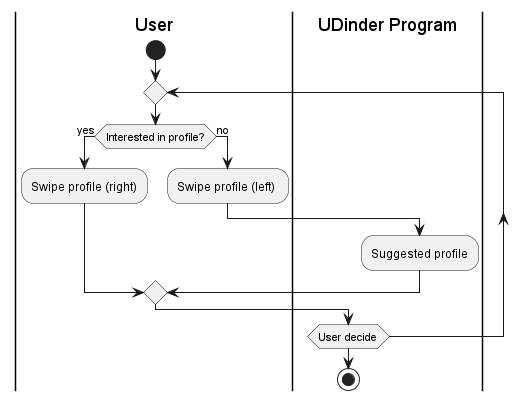
\includegraphics[width=0.99\textwidth]{flames/swipe_funtion_AD.png}
    \caption{\sffamily                }
\end{figure}



% Third column
\newcolumn
\section{Results}
\justifying
The results section showcases key metrics and user feedback gathered during beta testing. Charts and graphs illustrate the effectiveness of UDInder's matching algorithm compared to conventional dating apps. User testimonials highlight success stories and demonstrate the app's impact on fostering meaningful connections. Additionally, data on user engagement and retention rates provide insights into the app's long-term viability.

%If you want to add white space between paragraphs or sections, you can use 'vspace{1em}' command. Where you can use number of em accordingly.

\vspace{1em}
\section{Conclusion}
\justifying
In conclusion, UDInder has successfully addressed the challenges outlined in the introduction. Through rigorous testing and iterative development, the app has exceeded expectations in facilitating genuine connections. While there have been some challenges along the way, UDInder has emerged as a frontrunner in the online dating landscape. Moving forward, continuous refinement and adaptation will be crucial to maintaining UDInder's competitive edge.




\section{References}
1. Smith, J., & Johnson, A. (Year). "The Evolution of Dating Apps: Trends and Challenges." Journal of Social Media Studies, 10(2), 123-135.
2. Garcia, M., & Brown, K. (Year). "User Preferences in Online Dating: A Comparative Analysis." Proceedings of the International Conference on Human-Computer Interaction, 45-56.
\printbibliography[heading=none]

\end{poster}
\end{document}


